\chapter{Workflow}\label{chapter1}

In this project, I was required to build a microntroller model refered to a part of PIC16F84A, with VHDL language.
I used synthesizable VHDL to design and describe the circuit. The VHDL description comes from the course exercise 6.
According to the datasheet of PIC16F84A microntroller, the execution of an instrution could be devided into 4 phases:
\begin{enumerate}
  \item Fetch instruction from memory and decode it as arithmetic command and operand(if needed).
  \item Catch operand from memory, which is the result from the previous stroage.
  \item Do computation according to the arithmetic command.
  \item Write the result into memory address and register.
\end{enumerate}

After the VHDL description was done, I used Modelsim HDL simulator to do the simulation and verfication of functionality,
meanwhile debugging the errors and warnings.After the simulation and verfication were done, I followed the instructions to do synthesis, palce-and-route as well as
final verfication which will be presentated in the follwing sections. 


\section{VHDL description} 
The VHDL description of PIC16F84A are refered to the exercise 6 which consist of ALU entity for arithmetic operation,
RAM entity for memorable storage, MUX for Multiplexer and Finite State Machine(FSM) for finite state control.
As the microcontroller's behaviour is stepped by clock, the execution of one instruction will take max four cyles.
To make design easier, I used a finite state machine to implement the steps and named then as iFetch, Mread, Execute and Mwrite.
The input were assumed as 14-bit logic vecotr, in which from bit 13 downto bit 7 stands for arithmetic instruction,
while the part from bit 7 to bit 9 decide bit select and the part from bit 0 to bit 6 are address to write into memory.
For each arithmetic instruction, I created the relative functions and collected them in package "Instructionset".  
Then after one clock cycle, FSM entity tries to decode the instruction. 
It requires function ``string\_to\_instruction'' to get arithmetic instructions and send the signal to ALU entity. 
Then ALU will do computation of operand from command and thr ``operand\_array'' in RAM and return the result to FSM. 
Meanwhile, during one clock cycle, FMS's status has changed from Execure to Mwrite and increase program counter(PC)
by 1. FSM enables the writing to the ``operand\_array'' in RAM and return to the iFetch state in the next clock state.
In this process, MUX plays role to decide the source of result written to RAM depending on the instruction type which is indicated by
message from bit 13th to 12th. If it is byte or literature operation, result shall be wrriten to memory. If the result is bit type,
then the result shall be written to register.
\section{Interface Construction}
During this step, I refered to the example code of SPI interface which consist of a chain of Digital Flip-Flop connecting to n-bit register.
The VHDL code from exercise originally cannot be utilzed for synthesis because the test bench connectes all components but not synthesizable at all.
So I have to modify the test bech file into an interface connecting each components together and split the test part as a new test bench to 
do simulation and verfication. In this interface architecture, I should keep the port map of entities created and the necessary process.
 As I realized the importance of this step after browsing the instruction, I took two days to finish it.

\begin{figure}[!h]
    \centerline{\includegraphics[width=15cm]{./Figures/microcontroller\_interface.png}}
    \caption{microcontroller interface\label{fig00} }
\end{figure}

I declared a microntroller\_inteface has:
\begin{enumerate}
  \item generic
  \begin{itemize}
  \item depth: memory size
  \item length: instruction size
  \end{itemize}
  \item port
  \begin{itemize}
  \item clk: clock input
  \item rst: reset input
  \item instrwr: input enable writing to instruction
  \item PC\_tot: input total number of instructions
  \item instrution\_in: input instruction, string type
  \item opcode\_status: output FMS state
  \item statusOutput: output arithmetic status
  \item resultOutput: output arithmetic result
  \item addr: output current memory address 
  \end{itemize}
\end{enumerate}



\section{Test Bench}
Except the signals for components connection, there are four signals assign to input and output as concurrent process statement.
Base on that, I created a new test bench called ``ALU\_tb'' to do the functionality test.
There are two process in the test bench: ``clk\_finite'' and ``Reading\_text''.  ``clk\_finite''  will provide
finite length of clock input and enable reset originally for a while to initalize the signals. ``Reading\_text'' will 
firstly set instrwr as 1, reading the text lines from input file until the end, storing the instruction into memory via instruction\_in and increment PC\_tot.
After the reading is done, process set instr\_wr as 0, and write the output when the FSM status turns to be Mwrite. The output file will show
address, arithmetic result, arithmetic status.

\begin{figure}[!h]
    \centerline{\includegraphics[width=15cm]{./Figures/alu\_tb.png}}
    \caption{Test Bench \label{fig01} }
\end{figure}

\subsection{21st May}
On the original test bench, I merge the signals for address, operation\_wr, 
instruction\_wr on both RAM and FSM side because they shall not be separated on the test bech level. 
As I suppose, RAM accepts to store the instruction line from text file, and the enable port is instr\_wr, 
controlled by external signal. Once the reading process finished, the instr\_wr should be disabled and finite state machine started to extract, 
decode, computing and output result. So the op\_wr is controlled by finite state machine itself. Although the instr\_wr signal is transferred to both RAM and FSM, 
as long as it is disabled, the FSM should not work.  Similarly since the op\_wr is controlled by FSM, RAM won’t record the result as long as the op\_wr is disabled.

Simulation in Modelsim:
\begin{figure}[!h]
    \centerline{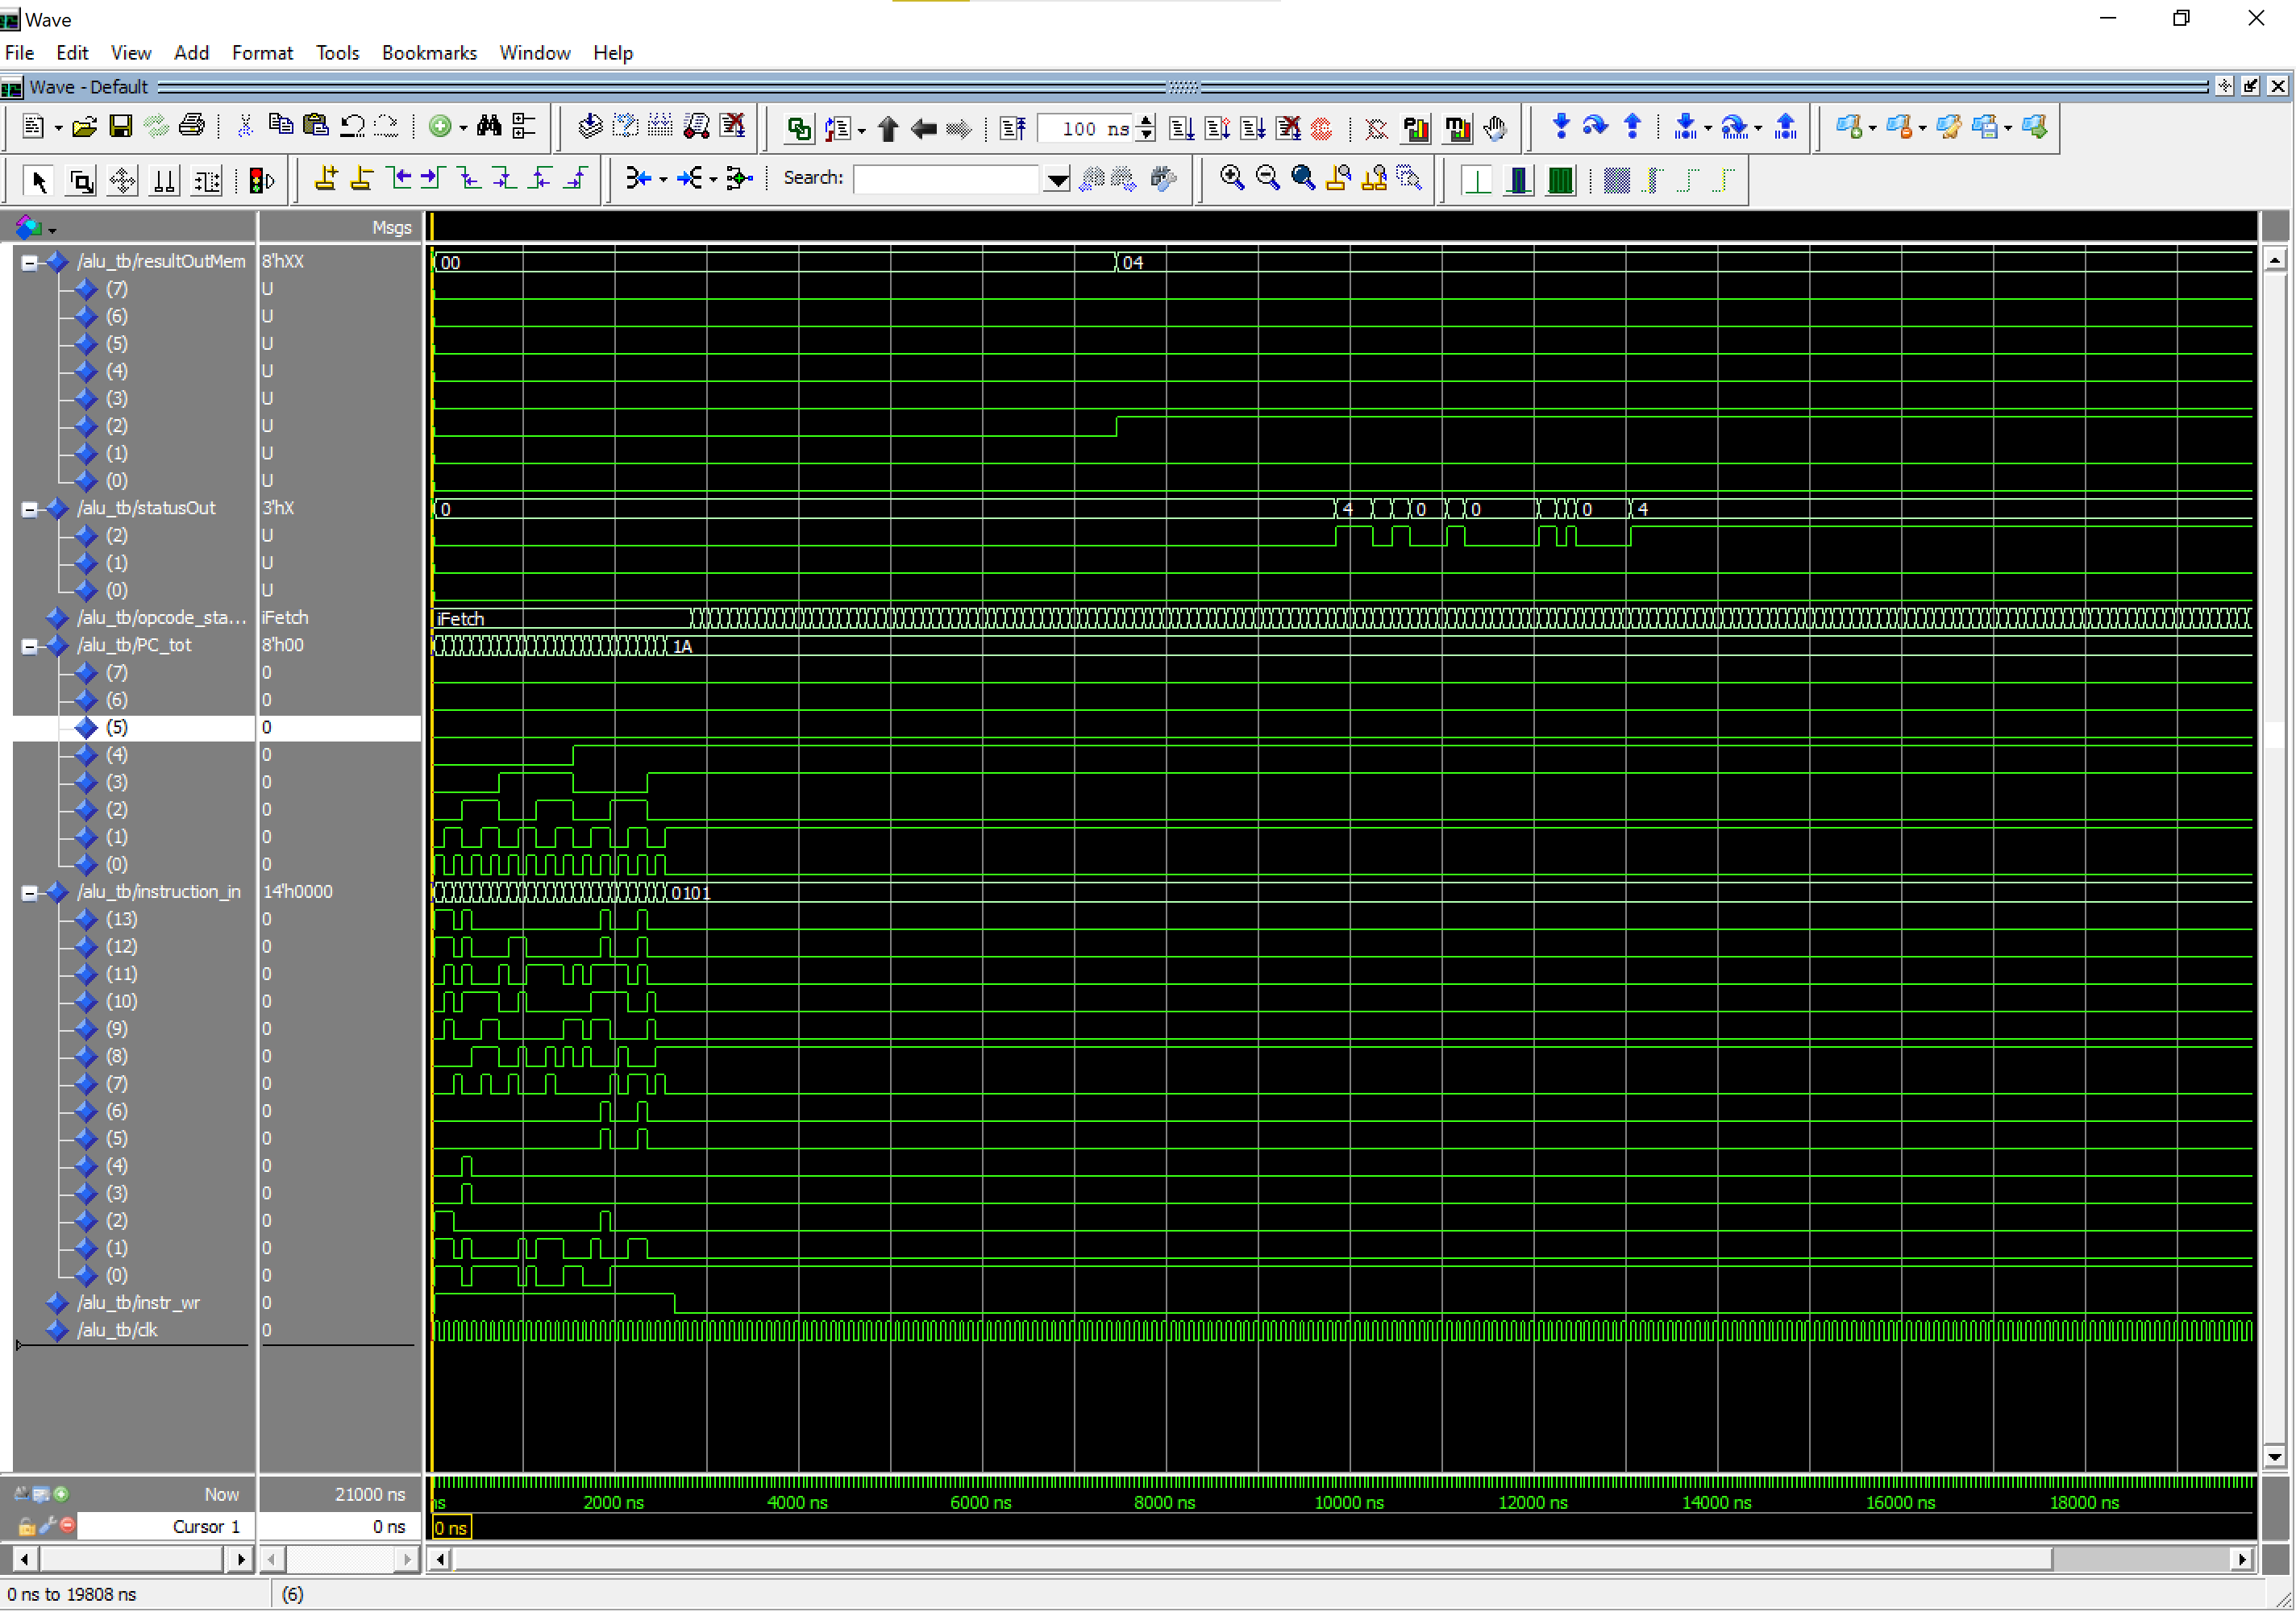
\includegraphics[width=15cm]{./Figures/waveform_modelsim.png}}
    \caption{Modelsim Simul and verfication \label{fig1} }
\end{figure}

As the picture shows that, the process starts by reading the instructions when the ``instruction\_in''
shows active, and then ``instr\_wr''was pulled down and ``opcode\_status'' become actvive too because the FSM
is working now. So the resultOut and statusOut give the output. Currently I could declare that
the computation result is as expected and the VHDL description is ready to do synthesis.

\section{Synthesis}
Synthesis process will convert the VHDL description into a gate-level netlist which describe the interconnection of
logic gates. In this process I used Synopsys Design Compiler(DC). 
\subsection{21st May}
I review the dicussion history on Slack channel and found that the warnings of latches might happen and I should
check it before the synthesis. To avoid latches, I checked all palces with conditional logic such as if-else and case-when.
I should declare the assignment for the situation if condition is not met or the other situations in case-when. Besides, if the case-when
take enumerate type condition, the ``when others=>'' are not needed or elaboration will rise alerts.
After that synthesiswill add desgin constraints like speed and operating conditions. Designer compiler will return a gate-level list
which uses the process vendor's library currently. Then we use Formality to do static verfication of functionality which compares the 
netlist created and the original VHDL description. The intention is to ensure that the logic should be equivalent on two different language
description.

\begin{figure}[!h]
    \centerline{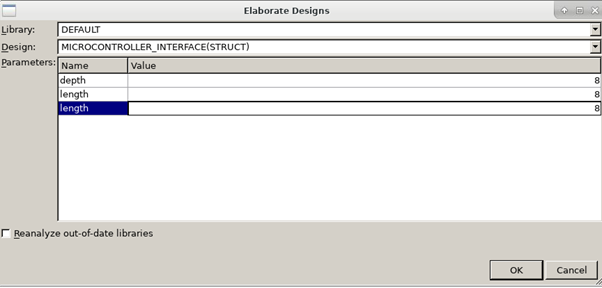
\includegraphics[width=15cm]{./Figures/elaboration.png}}
    \caption{Elaboration has redundant parameter \label{fig2} }
\end{figure}

\subsection{22nd May: Analysis, Elaboration}
When I used Design\_Vision, I should make sure the ``microcontroller\_interface.vhd'' the top level file is the first to add, in other words,
the top 1 in list. The order of other VHDL files are not matter even if they used each other as package(like ``Instructionset.vhd'').
After I loaded vhdl files, it was time to do elaboration. I found that the value for length delcaration are generic parameters instead of
constant parameters. So I went back to modify the VHDL files to removed the constant number ``N'' and replace it with ``length''. I make ``length'' and
``depth'' as generic parameters in all VHDL files. Finally when I come back to elaboration, I found that the parameters had one extra ``length''.
I still don't understand it but finally I moved the unecessary generic parameter from ALU and MUX entity, and here is no redundant parameter.


\subsection{23rd May: Constraint definitions, Compilation}
During the compilation, the system alerts that ``the inital value for signal `xxxxx' is not supported for synthesis. Presto ignores it. ''
So I removed all initial vlaue for signals and variables. It created another issue that circuit behaviour might have mestable status if some signals are
not initalized. Then I noticed that I can initalize them all in rest session. To do this, I went back to modify the entities architecture that 
in their process sensitive with rst, all signals are assigned with initial value. And the test bench could define 1/20 running time in the begining as reset phase. 

\subsection{24th May}
Today I am still in Elaboration session, and spent time to reduce the warnings in FSM. I found that in case conditional process for FSM, it would be best to declare
the assignment to a signal in all situations, or it will make mestable status too. For signals which requires no operation in other phases, I should move the assignment line
to another synchronous process which is triggered by clock and keep checking current stauts of FSM. I also removed the length defiend in package file because the generic
parameters ``length'' and ``depth'' might be variable.
I also noticed that the system sent many notifications about FlipFlop phenomenons in each entities. I asked question in Slack and assistant professor supposed it as out of problem.

\begin{figure}[!h]
    \centerline{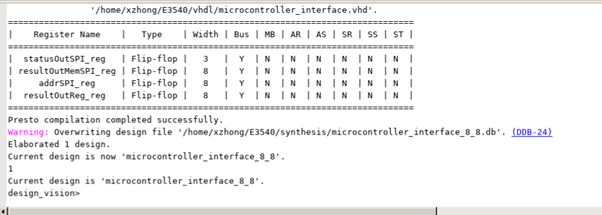
\includegraphics[width=15cm]{./Figures/elaborationWarning.png}}
    \caption{FlipFlop notification \label{fig3} }
\end{figure}

When I configure the drive strength and load to input and output ports, I found that Design\_Vision cannot recognize the ports as long as 
they are multibi array. And the constraints check will rise the area violoation instead of power violation mentioned in instruction because we set: 
``set\_max\_area 0''. Assistan professor supposed it as normal situation.

In max transition session, the violation happens with Net points n835, n8337, n8339 which are related to B0 bit. As I know, B is the input of
ALU to accept the result from register and it will be sent to arithmetic functions in Instructionset entity. 

In Static verification session, the Synopsys Formality checks the logic of VHDL code and netlist created from DC. 
When I set top design among the vhdl files loaded, I met another error:
\begin{itemize}
\item \textbf{Error: unsuppressed RTL interpretation messages} 
\item \textbf{Failed to set top design to microcontroller\_interface}
\item \textbf{Warning: Out of range write possible, 
may cause simulation and synthesis mismatch. 
(Signal: instruction\_array Block: RAM.rtl/state\_reg File: 
/home/xzhong/E3540/vhdl/RAM.vhd Line: 53) (FMR\_ELAB-146)}
\item \textbf{Warning: Index may take values outside array bound, 
may cause simulation mismatch .. (Signal: instruction\_array Block: RAM.rtl/state\_reg File: 
/home/xzhong/E3540/vhdl/RAM.vhd Line: 55) (FMR\_ELAB-147)}
\end{itemize}

I Gooled the warning content and found that it happens when we use integer as counter to address the memory storage.
So the solution is to change the program counter type to std\_logic\_vector and convert it to integer when needed. 

\section{Palce and route}
\subsection{25th May}
In previous process, I saved the TCL script of DC and Formality, and used to automate the process to do synthesis.
It saved much time for me to debug the potential issues in VHDL files.  
 Today I continue to do place and route in Encounter. The problem is that Encoutner's pin editor has fixed-size window
 while the OK button is below the desktop, so I cannot confirm the settings to the ports. So I have to use Innovus.
 I foudn that the default.view can be loaded in Innovus. Definitly it saved much time and energy. When I did the power planning,
 the console warnned that the VDD and VSS did not exist. The root cause is in the session to specify the floor plan, the distnace between
 core and margin was not valid for some reasons. Ater I specified the floor plan again, the issue had gone. In this process I found that 
 console is quite useful to monitor the process while UI window is not such important.

\begin{figure}[!h]
    \centerline{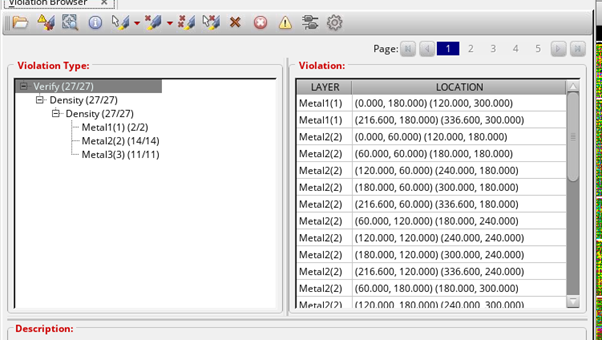
\includegraphics[width=15cm]{./Figures/MetalFilling.png}}
    \caption{Browse the verification result of metal density \label{fig4} }
\end{figure}

After Tiling, I found that several metal layers had violation. So I inserted OPC metal
fill shapes on the Metal1, Meta2 and Metal3. After that I verified the metal density again, the layout
still had Metal2 and Metal3 violated.

\section{Static verfication and timing analysis}
\subsection{26th May}
After I finished the static verfication and timing analysis, the final result is like below:

\begin{figure}[!h]
    \centerline{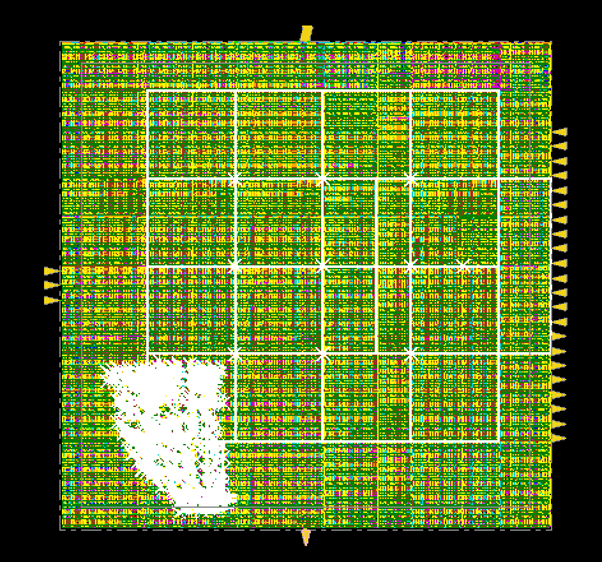
\includegraphics[width=15cm]{./Figures/FinalResult}}
    \caption{Final layout\label{fig5} }
\end{figure}

%This is how to insert equations.
% \begin{align}
%   H(0)& =-g_mR_L=\\
%   A_0[dB] &\approx 26dB\label{eq:approximation}
% \end{align}
%
